\documentclass{article}

\usepackage{listings}
\usepackage{graphicx}
\usepackage{color} %red, green, blue, yellow, cyan, magenta, black, white
\usepackage{amsfonts}
\usepackage{mathtools}

\newcommand\mat[1]{\mathcal{\underline{#1}}}

\definecolor{mygreen}{RGB}{28,172,0} % color values Red, Green, Blue
\definecolor{mylilas}{RGB}{170,55,241}
%% Preamble done!
%% Begin document
\begin{document}
\lstset{language=Matlab,%
    %basicstyle=\color{red},
    breaklines=true,%
    morekeywords={matlab2tikz},
    keywordstyle=\color{blue},%
    morekeywords=[2]{1}, keywordstyle=[2]{\color{black}},
    identifierstyle=\color{black},%
    stringstyle=\color{mylilas},
    commentstyle=\color{mygreen},%
    showstringspaces=false,%without this there will be a symbol in the places where there is a space
    numbers=left,%
    numberstyle={\tiny \color{black}},% size of the numbers
    numbersep=12pt, % this defines how far the numbers are from the text
    emph=[1]{for,end,break},emphstyle=[1]\color{red}, %some words to emphasise
    %emph=[2]{word1,word2}, emphstyle=[2]{style},    
}
\label{Cover}
	\begin{center}
	\large{ECE-5554 Computer Vision: Problem Set 1}
	\vfill
	Murat Ambarkutuk \\ murata@vt.edu
	\vfill
	Mechanical Engineering Department,\\ Virginia Polytechnic Institute and State University
	\vfill
	\today
	\end{center}
\pagebreak 
\large{Answer Sheet}
\label{Short Answer Problems}
\section{Short Answer Problems}
\begin{enumerate}
	\item
	\item 
	$$\vec{I} = \begin{bmatrix} 0 & 0 & 1 & 1 & 0 & 0 & 1 & 1\end{bmatrix}
	, \vec{f}= \begin{bmatrix} 1 & 1 & 1\end{bmatrix}$$
	\begin{equation} 
	\begin{split}
	\vec{H} & = \vec{I} \ast \vec{f} \\
	& = \begin{bmatrix} 0 & 1 & 2 & 2 & 1 & 1 & 2 & 2 \end{bmatrix}
	\end{split}
	\end{equation}
	\item
	\item
	\item
	\item 
	\begin{enumerate}
		\item Pre-processing (Preparation)
		\begin{enumerate}
	    	\item 
		\end{enumerate}
		\item Processing (Analysis)
		\begin{enumerate}
	    	\item 
		\end{enumerate}
		\item Post-processing (Interpretation)
		\begin{enumerate}
	    	\item 
		\end{enumerate}
	\end{enumerate}
\end{enumerate}
\pagebreak

\label{Programming Problem (Seam Carving)}
\section{Programming Problem (Seam Carving)}
\begin{enumerate}
	\item 
	\begin{enumerate}
		% subplot would be good 
		\item
		\item \\
		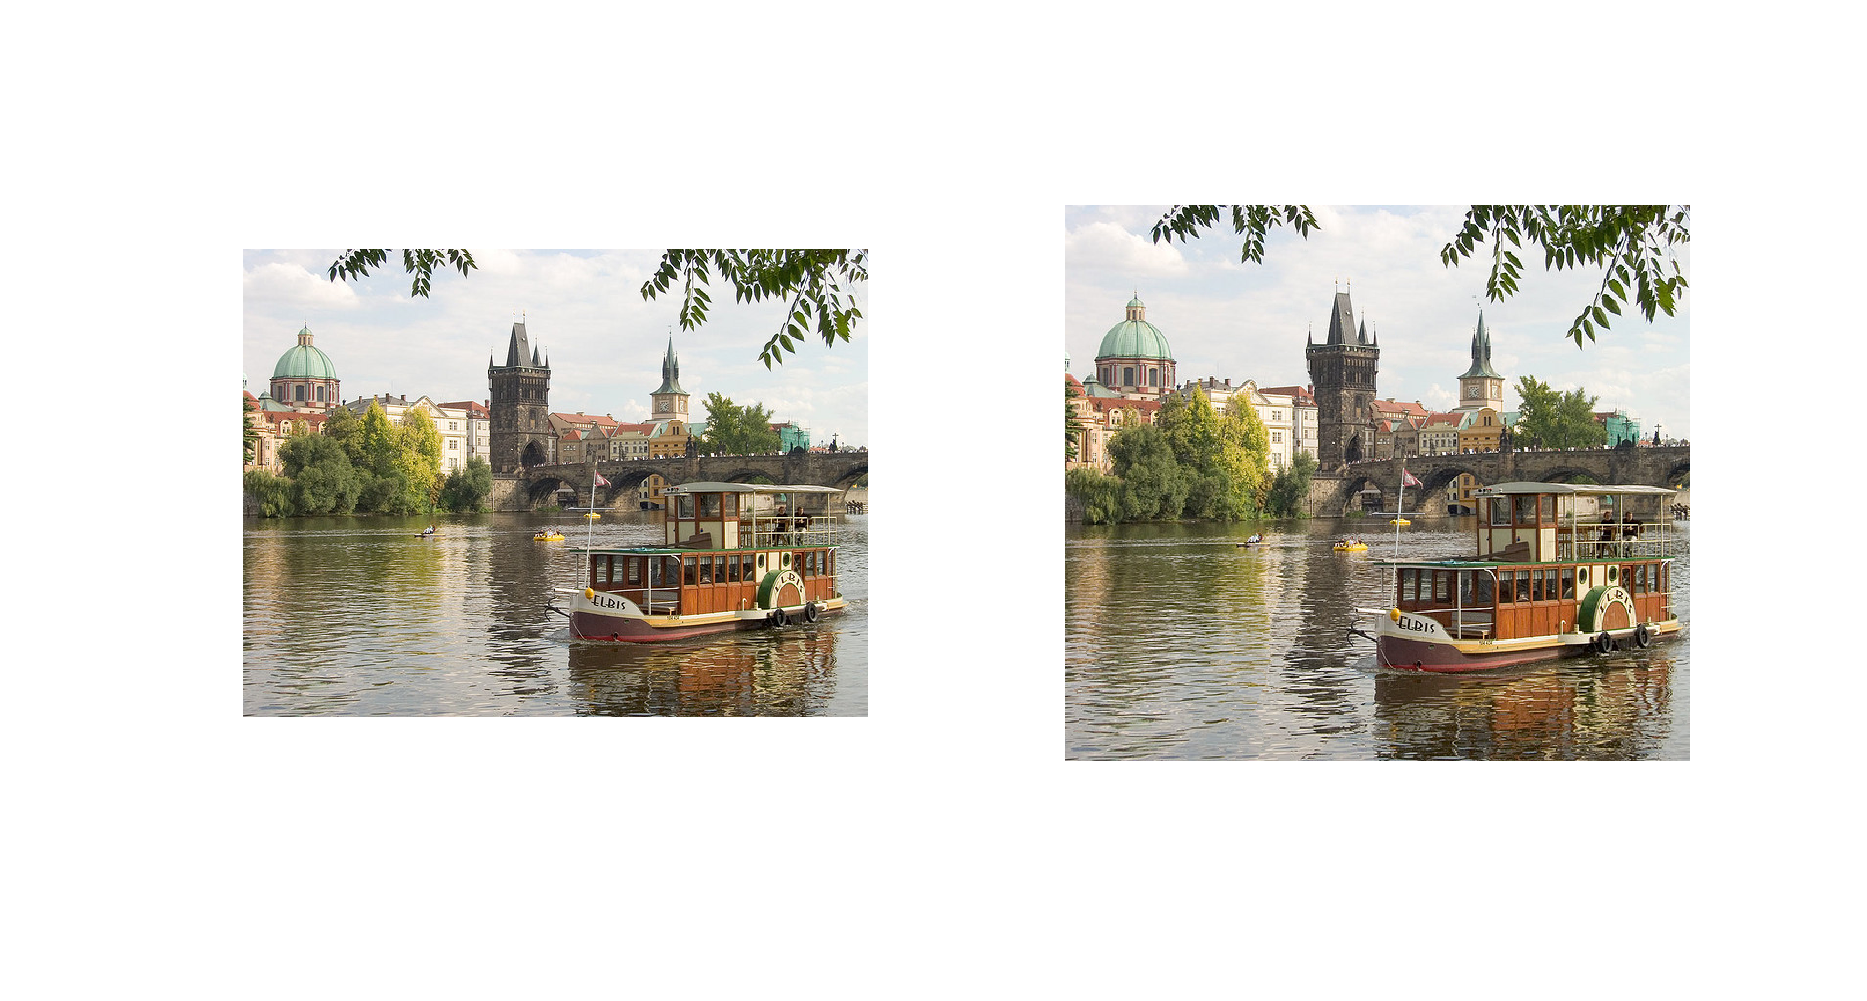
\includegraphics[width=\linewidth]{../matlab/outputPrague.png}
		\item
		\item
		\item 
	\end{enumerate}
	\item
	\item
	\item
	\item
	\item 
\end{enumerate}
\pagebreak

\label{Extra Credit}
\section{Extra Credit}
\begin{enumerate}
	\item
	% \setcounter{enumi}{4}
	\item 
\end{enumerate}
\end{document}
